\begin{figure}[!htb]
\begin{center}
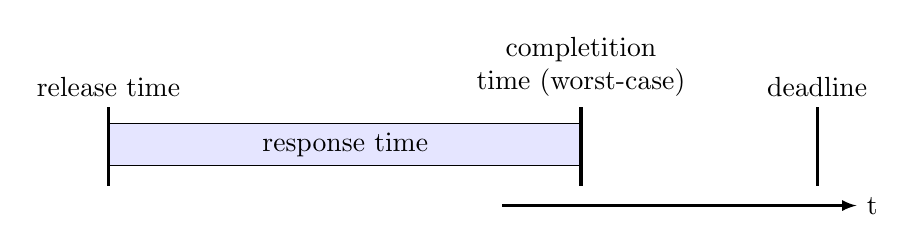
\begin{tikzpicture}

\node at (0,0.25)[rectangle, draw=black, fill=blue!10, minimum height = 0.5cm, minimum width = 6cm, anchor=south west] (resptime) {response time};
\draw[black, very thick, solid] (0,0) -- (0,1) node [above] {release time};
\draw[black, very thick, solid] (6,0) -- (6,1) node [above, text width=4cm, text centered] {completition time (worst-case)};
\draw[black, very thick, solid] (9,0) -- (9,1) node [above] {deadline};

%\node (rtlabel) at (5,-1.5) {response time};
\begin{scope}[>=latex]
	%%\draw [thick, ->] (rtlabel) to [bend left=45] (resptime.center);
	\draw[black, thick, ->] (5,-0.25) -- (9.5,-0.25) node [right] {t};
\end{scope}
\end{tikzpicture}
\end{center}
\ifreport
\caption{response time of real-time task}
\fi
\label{fig-rt-task-param}
\end{figure}
